% eltonPHYS4699.tex
% $Author: predrag $ $Date: 2018-07-25 16:48:43 -0400 (Wed, 25 Jul 2018) $

        \newif\ifdraft
%\drafttrue              % For draft version, commented
\draftfalse            % For final version, uncomment this

% JRE started LaTeX edits                Jan 18 2007
% PC created project LaTeX template         Jan 13 2007

% http://publish.aps.org/esubs/revtextips.html

 \documentclass[pre,twocolumn,groupedaddress]{revtex4}
% \documentclass[pre,preprint,groupedaddress,showpacs,showkeys]{revtex4}

\input defs         % all definitions in defs.tex
                \begin{document}
                \title{
An exploration of moderate \Reynolds\ plane Couette turbulence
                }\author{
John R. Elton            }
        \email{
gtg960p@mail.gatech.edu
              }
        \affiliation{
School of Physics\\
Georgia Institute of Technology, Atlanta, GA 30332-0430
                }
%               \date{\today}
               \date{April 29, 2007}

                \begin{abstract}
The {\tt channelflow} code~\cite{channelflow} for determining
equilibria and unstable periodic orbits of moderate \Reynolds\ plane
Couette turbulence is implemented and applied. A look at
modification of flow parameters and initial conditions has been made
to further investigate phase space properties for \pCf.

\end{abstract}
\pacs{95.10.Fh, 02.70.Bf, 47.52.+j, 05.45.+a}
\keywords{
periodic
orbits, chaos, turbulence, ???
    }
                    \maketitle

\noindent
{\bf Georgia Tech PHYS 4699:}\\
\underline{\bf CHAOS, AND WHAT TO DO ABOUT IT }\\
{\bf special problems project, spring semester 2007}


\section{\PCf}
\label{sec:PCF}

\PCf\ describes the motion of a fluid constrained by two long plates
moving in opposite directions (along the streamwise $x$ axis) at the
same constant speed. The distance between the plates in the
wall-normal $y$ direction is chosen to be 2, with one plate at 1 and
the other at -1.  Periodic boundary conditions are imposed on the
streamwise $x$ and spanwise  $z$ directions which allows for one
section of the flow to be analyzed.  Given a set of fluid constants
and initial conditions the Navier-Stokes equations may be solved
numerically to find the velocity field as a function of time (see
fluid notes, \refsect{sec:fluids}). One of the tools for performing
this task is the {\tt channelflow} code {\tt couette.cpp}
~\cite{channelflow} which works as outlined in
\refsect{sec:couette.cpp}. The velocity field $u(x,y,z)$ can be
expanded as a set of orthogonal basis functions \beq u(x,y,z) =
\sum{a_{n} \Phi_{n}(x,y,z)} \eeq where the basis set $\Phi_{n}$
spans the same finite-dimensional function space as the chosen
$N_{x} \times N_{y} \times N_{z}$ grid. Because of the periodicity
in $x$ and $z$ the basis functions are of the form \beq \Phi_{j,k,l}
=  \phi_{l}(y) e^{2 \pi i(jx/L_{x} + kz/L_{z})} \eeq \PC{doesn't
$\phi_{l}(y)$ depend on $j,k$? Maybe not...}
 \JRE{I think the idea is that in the decomposition the subscripts
 j,k are associated with the Fourier modes in x and z and the
 subscript l is the only one needed to define the polynomial in y.}
 where
j and k are Fourier modes and $\phi_{l}$ is a polynomial in $y$
which satisfies the boundary conditions. The coefficients are
represented in {\tt channelflow} as \verb"ColumnVectors".  For
computations it is often necessary to write the velocity fields as a
DNS spectral expansion called a {\verb"FlowField"} object, \beq
u(x,y,z) = \sum_{jkl}{\hat{u}_{jkl}} T_{l}(y) e^{2 \pi i(jx/L_{x} +
kz/L_{z})}, \eeq where the spectral coefficients $\hat{u}_{jkl}$ can
be converted back and forth from {\verb"FlowFields"}  to
{\verb"ColumnVectors"} through the functions {\tt field2vector} and
{\tt vector2field}.  Use of this is made in the program {\tt
couette.cpp} where one can compute the $L^{2}$ norm of the expansion
coefficients and it is the same as the $L^{2}$ norm of the velocity
field \emph{from} the laminar state. The $L^{2}$ norm $\|f\|$
(familiar Hilbert space from Quantum Mechanics) is defined for a
function f on a volume $V$ ~\cite{Holmes96} as \beq \|f\|^2 =
\frac{1}{V} \int_{V} |f|^{2}\,dx\,dy\,dz. \label{L2norm} \eeq

 \subsection{Program couette.cpp}
\label{sec:couette.cpp}

  The program {\tt Couette.cpp} is used to integrate
 {\pCf}
 from an initial field for a specified time. I outline here (with C++ notation) the important parts of this
 program.

  \noindent // Define flow parameters \\
  const Real Reynolds = 400.0; \\
  const Real nu = 1.0/Reynolds; \\
  const Real dPdx = 0.0; \\
  const Real Ubulk = 0.0;

Here we have the first important parameter inputs. The Reynolds
number \refeq{PCFRe} determines the viscosity of the flow. We also
see the incompressibility condition \refeq{incompr}.


 \noindent // Define DNS parameters \\
 flags.initstepping = CNRK2;


The numerical integration method is a combination of the
Crank-Nicholson and Runge-Kutta 2 methods.

 \noindent  // Define size and smoothness of initial disturbance \\
  Real spectralDecay = 0.3; \\
  Real magnitude  = 0.1; \\
  int kxmax = 3; \\
  int kzmax = 3;

The spectral decay number determines the rate at which the spectral
coefficient in $y$ decays back to the laminar state. The coefficient
$\hat{u}_{l}$ is defined as
\beq
|\hat{u}_{l}| = \mbox{rand}[0,1] *
(\mbox{spectraldecay})^{l}
\eeq
and thus we see that the dependence of
$\hat{u}_{l}$ on spectral decay number is the slope when
$\log |\hat{u}_{l}|$ is plotted against $l$.


  \noindent  // Construct data fields: 3d velocity and 1d pressure \\
  cout $\ll$ ``building velocity and pressure fields..." $\ll$ flush; \\
  FlowField u(Nx,Ny,Nz,3,Lx,Lz,a,b); \\
  FlowField q(Nx,Ny,Nz,1,Lx,Lz,a,b); \\
  cout $\ll$ ``done" $\ll$ endl;

  Velocity and pressure fields are created for the given box size
  $(N_x,N_y,N_z)$ as {\verb"FlowFields"} (3).


  \noindent // Perturb velocity field \\
  u.addPerturbations(kxmax,kzmax,1.0,spectralDecay); \\
  u *= magnitude/L2Norm(u);

After the initial {\verb"FlowField"} objects are set up the \\
perturbations are added and $u$ is updated.

    \noindent // for (Real t=0; t$\leq$ T; t += n*dt) { \\
    cout $\ll$ "         t == " $\ll$ t $\ll$ endl; \\
    cout $\ll$"       CFL == " $\ll$ dns.CFL() $\ll$ endl; \\
    cout $\ll$ " L2Norm(u) == " $\ll$ L2Norm(u) $\ll$ endl; \\
    cout $\ll$ "divNorm(u) == " $\ll$ divNorm(u) $\ll$ endl;

 These are the printed outputs that show up when the program is run.
$``t ="$
clearly shows the time step that the program is on.
 ``CFL" is a number related to the flow parameters which needs to be
 between 0 and 1. For most cases it takes a value around
 0.4 - 0.5.  It can be approximately given as $CFL \thickapprox \frac{\triangle t u}{\triangle
 x}$. ``L2Norm" (4) gives the distance of the solutions from laminar
 flow.  It is interesting to watch the variations in L2Norm as spectral decay number is varied.
  It always starts our at the value 0.1 and for large spectral decay rates goes quickly to
 0, but grows for decay rates $\sim 0.5$.
``divNorm" is a number which should be very close to
 zero, $O\thicksim 10^{-16}$.


\section{Wall law and Vertical Vorticity}
\label{sec:WallLaw}

 Upon reading Gibson's "Upper/lower/laminar branch" blog ~\cite{stability-spring}, I
found that for \pCf\ one may linearize the Navier-Stokes equations
about a base flow by letting \beq \vec{v} \rightarrow U(y) \hat{x} +
\vec{v}(x,t)\eeq where the base flow is $U(y) \hat{x}$. In this
approximation, how does the base flow respond to a variation in the
flow parameters? The theoretical approximation for the base shear
flow is the `Wall Law'. It predicts \beq U(y) \thicksim y \eeq
 for $y <10$ and
       \beq U(y) \thicksim 5 + 2.5*log(y) \eeq for  $y > 10$.
 Here I look at the Wall law program in {\tt channelflow}, which
computes the average velocity profile $U(y)$ of a pressure-driven
flow and compares it to the theoretical approximation for $U(y)$.
This program allows one to investigate the behavior of the base flow
and check that it remains fairly stable.

 The vertical vorticity, $\eta$, is defined by
\beq \eta = (\nabla \times \vec{v}) \cdot \hat{y}, \eeq
  so according to
 the following simple calculation, a `wall-law' base flow should contribute
 nothing to the vertical vorticity. That is,
the base flow should be  stable with respect to a variation in the
flow parameters.
  \beq \vec{U}(y) = y \hat{x}, \eeq
    \beq \nabla \times \vec{U} = \hat{x}(\frac{\partial U_{z}}{\partial
 y} - \frac{\partial U_{y}}{\partial z}) - \hat{y}(\frac{\partial U_{z}}{\partial
 x} - \frac{\partial U_{x}}{\partial z}) + \hat{z}(\frac{\partial U_{y}}{\partial
 x} - \frac{\partial U_{x}}{\partial y}) \nonumber \eeq
 \beq = - \frac{\partial U_{x}}{\partial
 y} \hat{z} = -\hat{z}, \nonumber \eeq
 \beq (\nabla \times \vec{U}) \cdot \hat{y} =\eta = 0. \eeq No vertical vorticity.
  This being the case, if one plots the mean velocity profile against y,
the theoretical approximation should be more or less returned
regardless of the
 magnitude of the parameters, though the parameters strongly affect the non-laminar
 part of the flow. This seems somewhat obvious, but it is a good check
 nevertheless. To check it I have run the {\tt wall-law} program and plotted
 results for several different cases in which the Reynolds number, the
 perturbation magnitude, and the spectral decay rate were varied against a base
 flow with no perturbations.
One can see from \reffigs{eltonFig:perturb1}{eltonFig:perturb2} that
despite considerable changes in the perturbation parameters and
Reynolds number, there is little deviation from the wall law. In
fact the perturbation changes are hardly even visible. One can see
the slight changes due to the variation in Reynolds number, but to
obtain even this small deviation, the Reynolds number was decreased
by an order of 100. This confirms the $\eta = 0$ calculation for the
mean base flow.


\begin{figure}[htbp]
(a)\includegraphics[width=0.40\textwidth]{walllawbase}
(b)\includegraphics[width=0.40\textwidth]{walllaw1}
 (c)\includegraphics[width=0.40\textwidth]{walllaw2}
  \caption{Variation in Re with perturbation magnitude = 0.01, decay rate = 0.01.
  (a) {Base flow}  (b) { Re = 4,000} (c) { Re = 40}}
  \label{eltonFig:perturb1}
 \end{figure}


\begin{figure}[htbp]
 (d)\includegraphics[width=0.40\textwidth]{walllawbase}
 (e)\includegraphics[width=0.40\textwidth]{walllaw3}
 (f)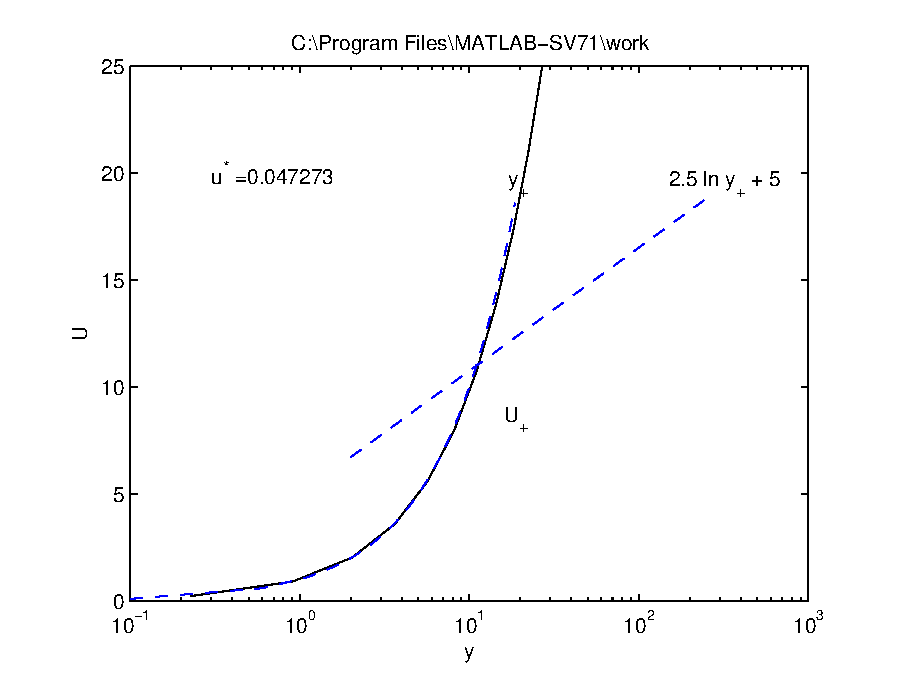
\includegraphics[width=0.40\textwidth]{walllaw4}
  \caption{Perturbation variations at Re = 40. (a) {Base flow}  (b) {Magnitude = 1.0,
  decay rate = 0.01} (c) {Magnitude = 0.01,
 decay rate = 0.1}}
 \label{eltonFig:perturb2}
 \end{figure}



\section{{\tt PCF-utils} methods and results}

 I have been able to produce some phase space
trajectories for random initial fields, and random initial
conditions along eigenvectors from \eqva. First I will document the
use of the various {\tt channelflow} programs for the phase space
flows, and then give some plots and results.

\subsection{How to implement}
The documentation and descriptions here are similar to those
provided in the {\tt PCF-utils} repository, but with specifics and
details to running on my machine.

\textbf{Method I : A random initial condition} \\
 1.) Create a random initial field. \\
This is done by the program {\tt randomfield} which takes the arguments
of box size, magnitude, and smoothness of field. To run: \\
./randomfield.x -Nx 48 -Ny 35 -Nz 48 -a 1.14 -g 2.5 -s 0.5 -m 0.3
urand.48.35.48 \\
where urand.48.35.48 is the output file name.\\
Random field satisfies the boundary and zero-divergence conditions.

 2.) From the initial field, integrate the Navier-Stokes equations. Program
{\tt couette} does
this for a specified time interval and saves the flowfield in
data/u1 as filename u1. The path data/u1 needs to be created before
running.
 To run: \\
./couette.x -T0 0 -T1 400 -o data/u1 -l u1 urand.48.35.48 \\
Program couette takes a rather long time to run.

3.) From a linearly independent set of fields on the trajectory,
create an orthonormal basis. Program {\tt makebasis} outputs this
set to
a specified directory. To run: \\
./makebasis.x -o basis1 data/u1/u10 data/u1/u110 data/u1/u120 data/u1/u130 \\
where \{u10, u110, u120, u130\} is the basis set.

4.) Project fields onto the basis set for a specified interval of
time. Program {\tt projectseries} inputs the basis and outputs to the
file u1.asc. To run: \\
./projectseries.x -T0 0 -T1 400 -bd basis1/ -Nb 4 -d data/u1 -ul u1 -o u1.asc

5.) With the file u1.asc at hand, all that is left is to load into
matlab and graph. In order to do this matlab needs to have {\tt
PCF-utils}
in its path. In the matlab window type: \\
path(path,'C:/cygwin/home/OWNER/workspace/
channelflow/PCF-utils') \\
Next load the file by entering: \\
load u1.asc \\
Finally to plot the trajectory enter: \\
plot3(u1(:,1), u1(:,2), u1(:,3));

\textbf{Method II : A random perturbation from an \eqv} \\
1.) Suppose we already have an \eqv\ point uUB, and an associated
eigenfunction, UBef1, such as for the \ubranch. Adding a
perturbation along the eigenfunction simply involves taking a linear
combination of the two (in which the perturbation coefficient is
small) using the program {\tt addfields}. To run: \\
./addfields.x 1 uUB 0.01 UB\_ef1 uUB\_0.01\_ef1 \\
where 1 and .01 are the coefficients. uUB\_0.01\_ef1 is the output
field.

2.) Now take this field uUB\_0.01\_ef1 close to the \eqv\ and go
back to step 2.) of method 1 to perform the integration, make the
basis set, project, and plot.


\subsection{Method 1 results: 3/22/07}
Using method 1 I have added trajectories for several different
random initial fields, see \reffig{eltonFig:random1}. \PC{
    can you mark the initial points in \reffig{eltonFig:random1}
    by small dots or circles, just to get a sense of which way the flow goes
   }The parameters I use in {\tt randomfield} are smoothness and
magnitude of the initial field. For \reffig{eltonFig:random1}(a),
 values of $s = 0.5$, $ m = 0.8$ are used. For
\reffig{eltonFig:random1}(b) I decreased magnitude to $m = 0.3$ and
smoothness to  $s=0.1$.

The difference in the plots for these varied values is quite
interesting. There is a similar dense area at about $y=0.15$.\PC{If
you have a suspect, $y=0.15$ is not enough. Please save a trajectory
point in the suspected region as an (informatively named) data set
in the subdirectory programs/data/, for John F. and Jonathan to plot
into their figures of unstable manifolds, to get a sense where your
suspect is in relation to other suspicious regions.
   }
More could be extracted from many more comparisons of nearby values
and longer integration times. There may be a particular value of
either of these parameters for which the structure of the \statesp\
flow changes quickly. \\
\begin{figure}[htbp]
  (a)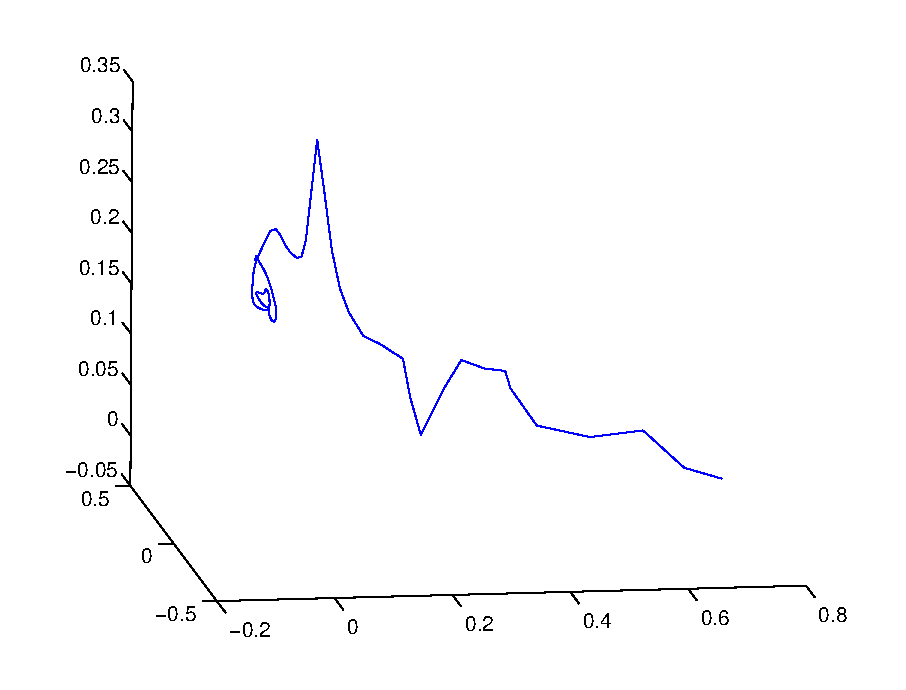
\includegraphics[width=2.5in]{plot2}\\
  (b)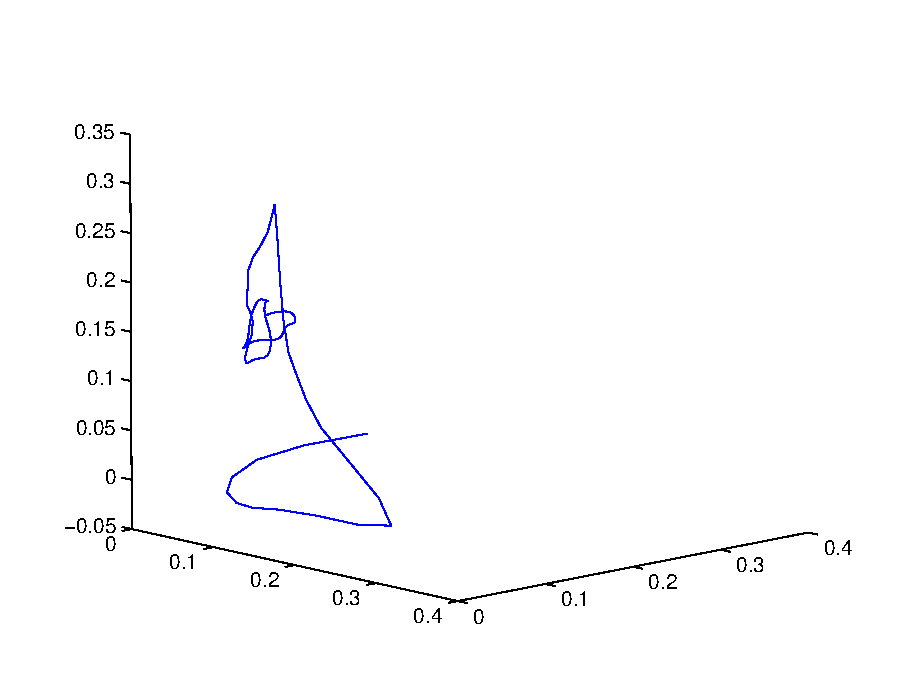
\includegraphics[width=2.5in]{plot3}
  \caption{Trajectories for a random initial
  condition for smoothness and magnitude
  values of
    (a) $ s=0.5 $,  $m=0.8 $, $T=100$
    (b)  $s=0.1 $,  $m=0.3 $, $T=100$
          }
          \label{eltonFig:random1}
  \end{figure}

\subsection{Method 1 results: 4/29/07}
\begin{figure}[htbp]
  (a)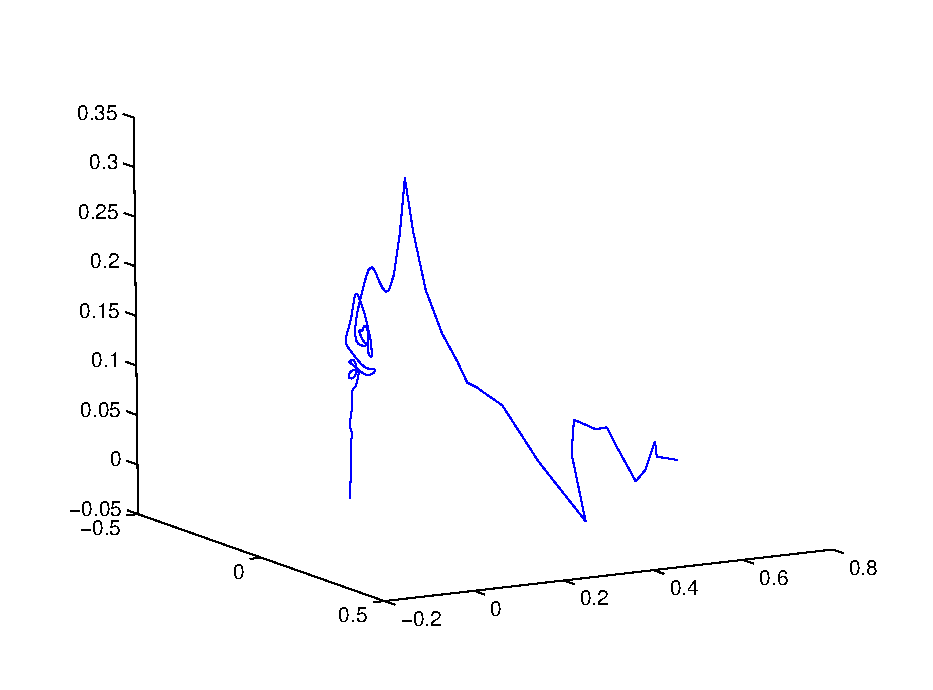
\includegraphics[width=2.5in]{plot5}\\
  (b)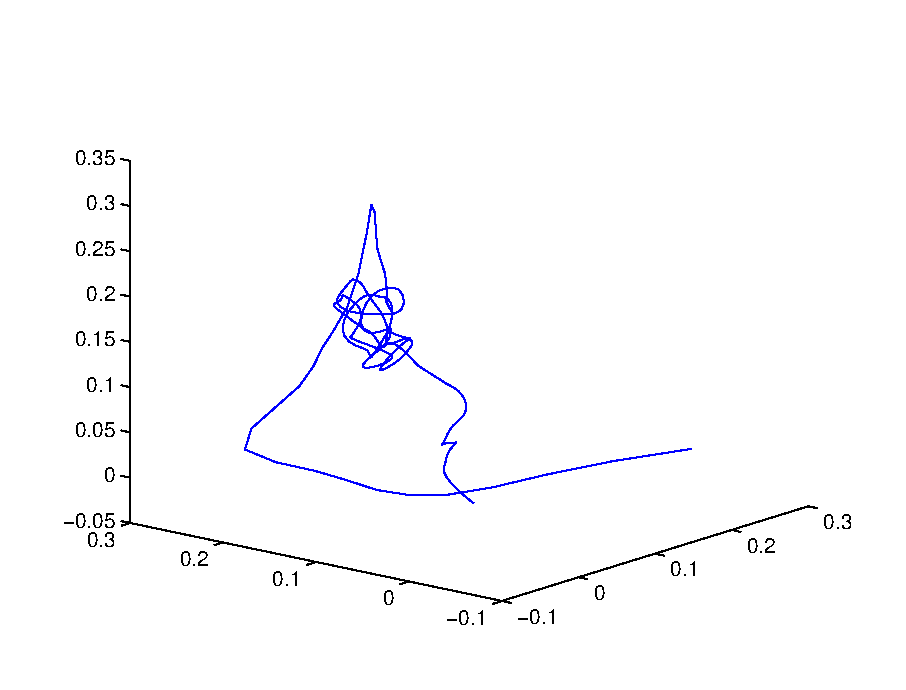
\includegraphics[width=2.5in]{plot4}
  \caption{Trajectories for a random initial
  condition for smoothness and magnitude
  values of
    (a) $ s=0.5 $,  $m=0.8$, $T=400$ - file {\tt u1.ff}
    (b) $s=0.1 $, $ m=0.3$, $T=400$ -  file {\tt u2.ff}
          }
          \label{eltonFig:random2}
  \end{figure}
  \begin{figure*}[htbp]
  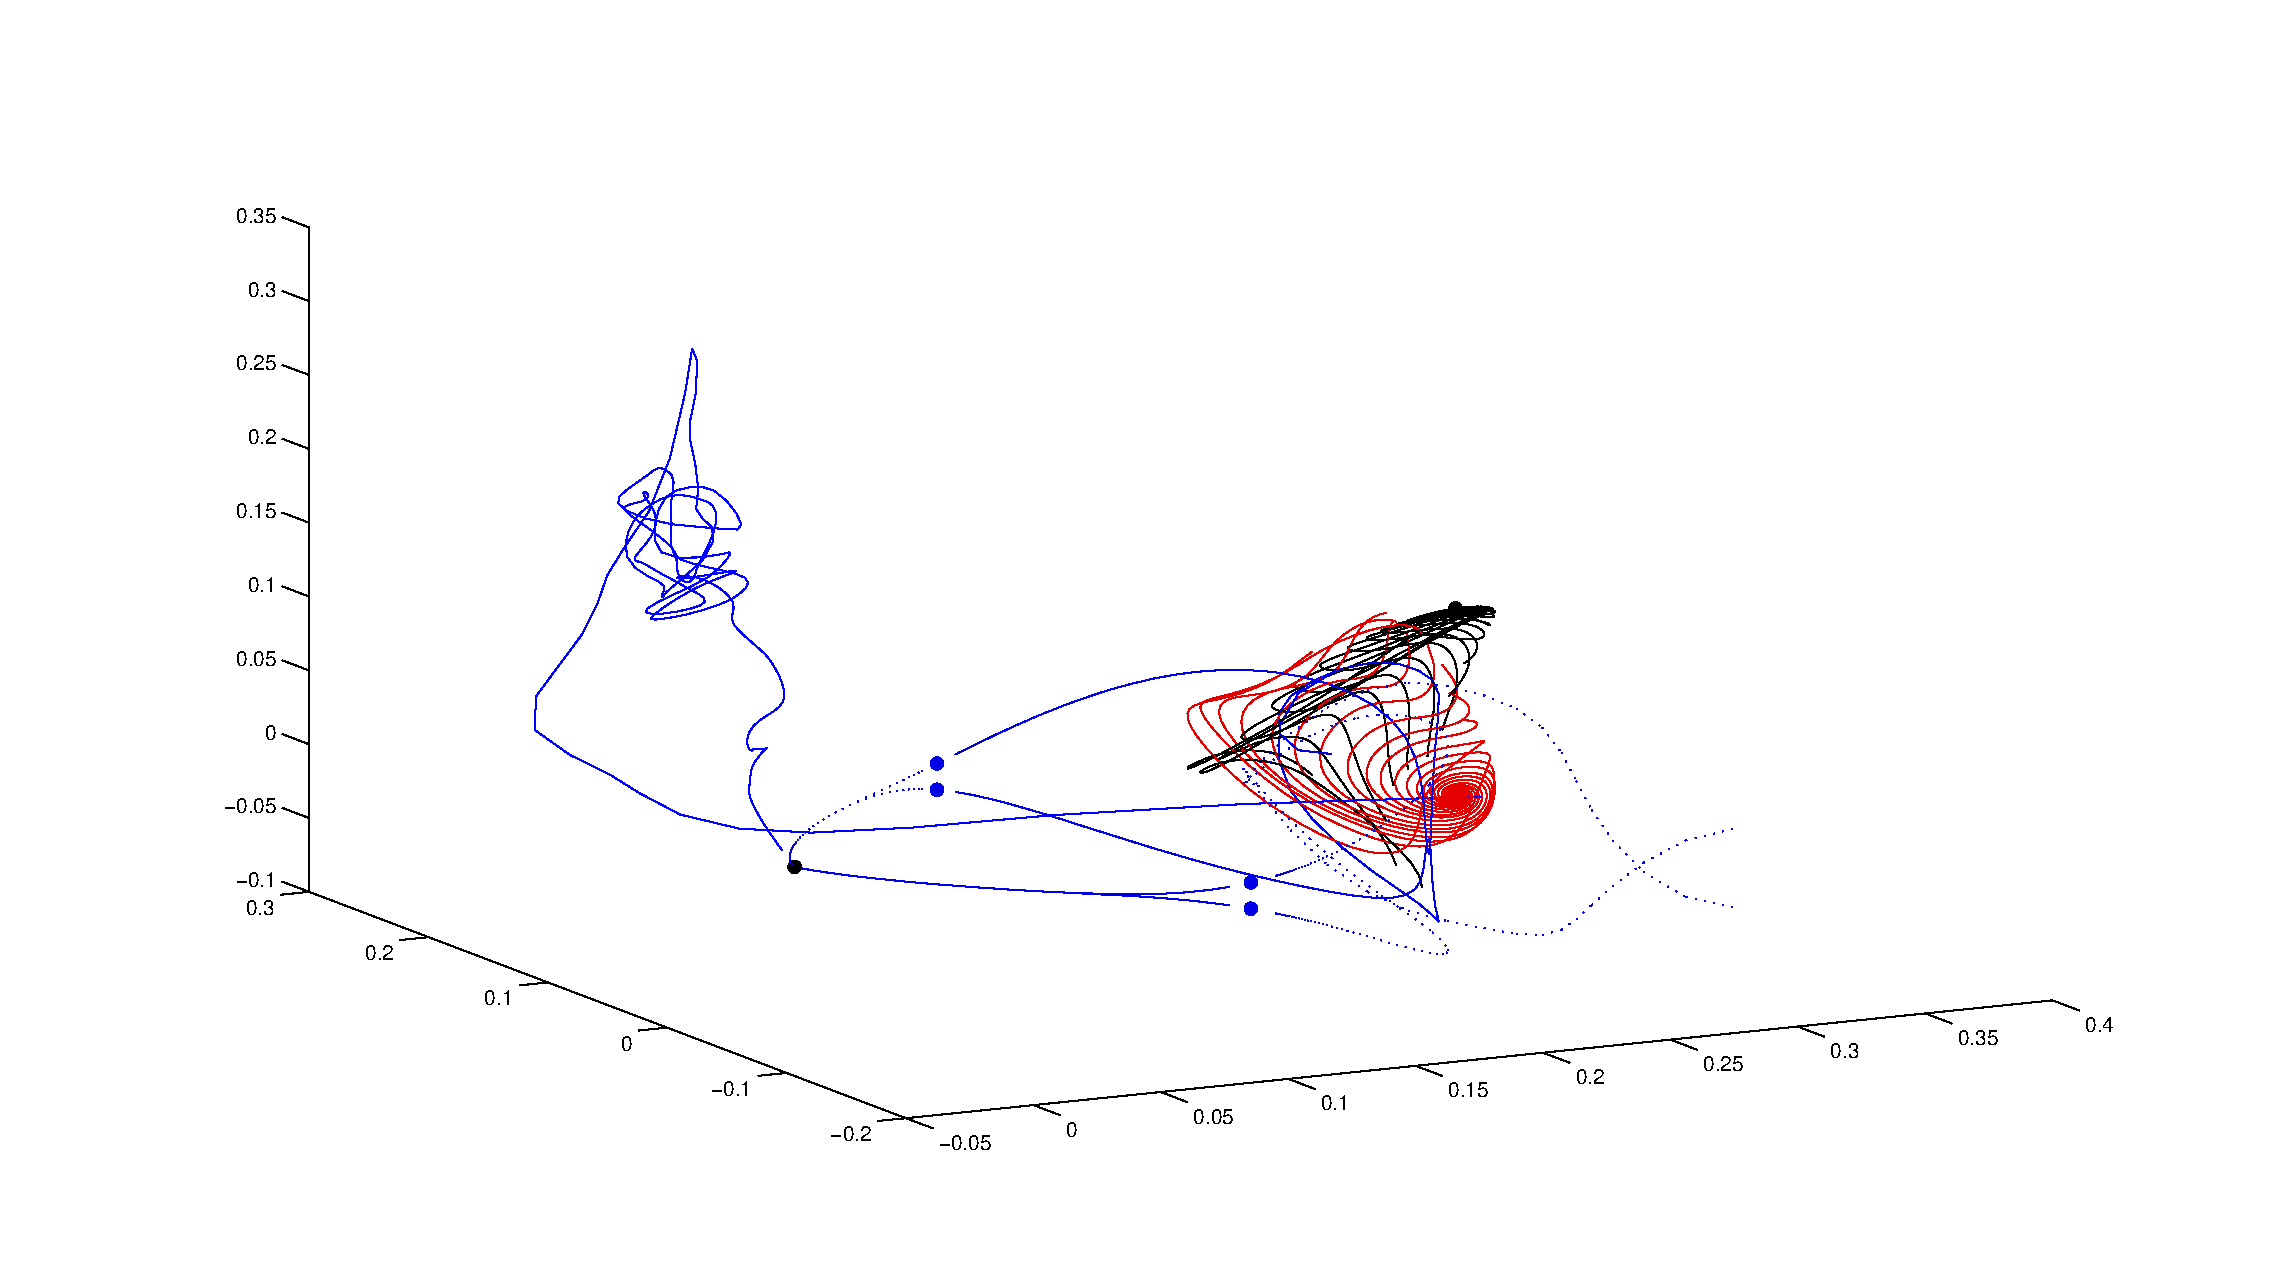
\includegraphics[width=5.0in]{u2andUB}
  \caption{UB and u2}
\label{UBu2}
\end{figure*}
Upon longer integration times of \reffig{eltonFig:random1} more can
be seen about the suspicious region in \reffig{eltonFig:random2}.
 I have attempted to bound this region by projection
onto the $xy$ and $yz$ planes to give the rough values $ 0.1 \leq x
\leq 0.15 , 0.15 \leq y \leq 0.2 , 0 \leq z \leq 0.05 $.  As can be
see from \reffig{eltonFig:random2}, upon running the time out to $T
= 400$ the trajectories do eventually leave this region, but not for
quite some time. It is curious that each random trajectory finds
this region and stays trapped for some time. This seems to suggest
that the region must be fairly strongly attracting. In \reffig{UBu2}
I have added \reffig{eltonFig:random2}(b) along with a phase space
plot of the upper branch in order to get a better feel for where
this region lies. In comparison with the upper branch plot my figure
is in an entirely different region of the space. There may be an
interesting behavior connecting the regions or possibly another
unstable manifold in the area near {\tt flowfield} u2.

\subsection{Method 2 results 4/29/2007}

Starting from Waleffe's {\ubranch}, as recomputed at higher accuracy
by Gibson ~\cite{PCFdata}, I have added plots for perturbations
along each of the 7 eigenfunctions in
\reffigs{eltonFig:UBefs1/old}{eltonFig:UBefs2/old}. The difficulty
is determining and computing an {\eqv} (I have used a precomputed
Waleffe's {\ubranch}) and deciding where to start. This having been
done already, I have the following in
\reffigs{eltonFig:UBefs1/old}{eltonFig:UBefs2/old}. The region
connecting the UB and the NB would be an interesting place to look
as it is a little less well understood. For this it would be
necessary to know which eigenfunction points in that direction. It
is necessary to compare these plots with previously computed data to
make sure they are sensible and to get more of a feel for what the
behavior means. The spiral behavior at the onset of (e) and (f)
would suggest a comparatively large imaginary part of the
eigenvalues for these two. \PC{large? it is always between 0 and
$2\pi$} \JRE{just in comparison with the other eigenvalues}Sure
enough, from Table 1 of Gibson's blog "\Statesp\ portraits of the
LB, NB, UB" ~\cite{state-space}, eigenfunctions (e) and (f) of
\reffig{eltonFig:UBefs2/old}) have eigenvalues $ \lambda = 0.01539 +
i(0.28418)$ which have much larger imaginary part than any of the
others.

In \reffigs{eltonFig:UBefs1/new}{eltonFig:UBefs2/new} perturbations
from the same eigenfunctions have been plotted only this time using
the \emph{same} basis for each. The chosen basis is one which
sustains typical upper branch behavior for the given flow
parameters. This allows for a comparison between these plots and
previously computed upper branch data in, for example, Gibson
~\cite{state-space}.


\newpage
% old eigenfunction figures
\begin{figure}[htbp]
  (a)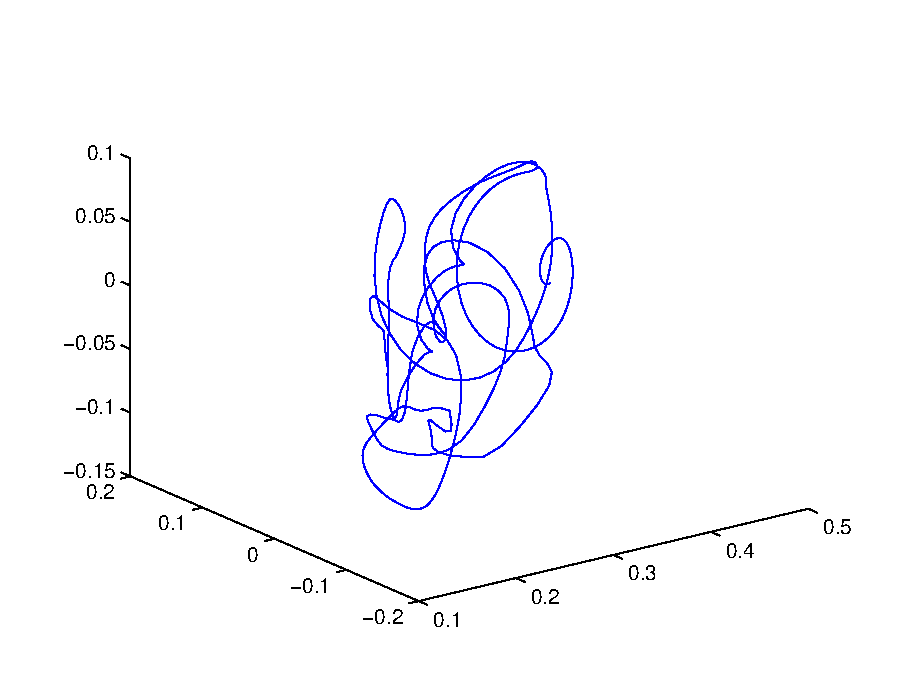
\includegraphics[width=2.5in]{UBef1}\\
  (b)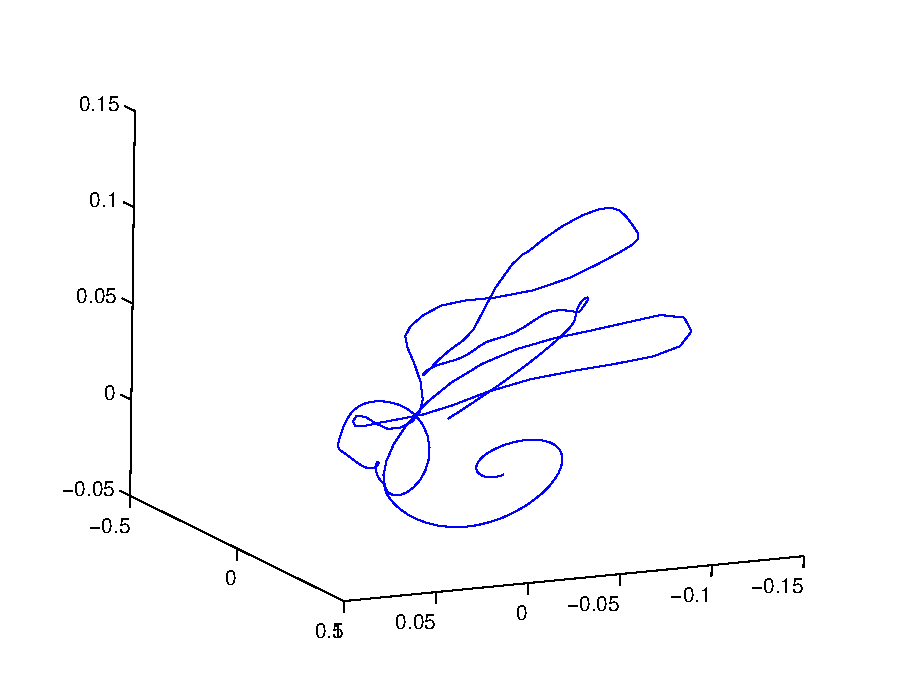
\includegraphics[width=2.5in]{UBef2}\\
  (c)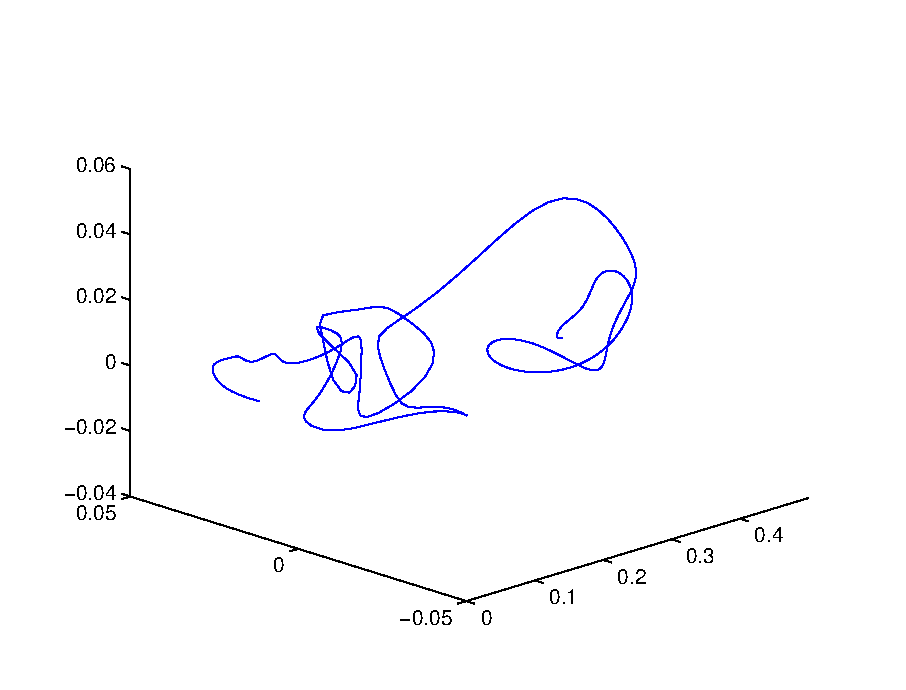
\includegraphics[width=2.5in]{UBef3}\\
  (d)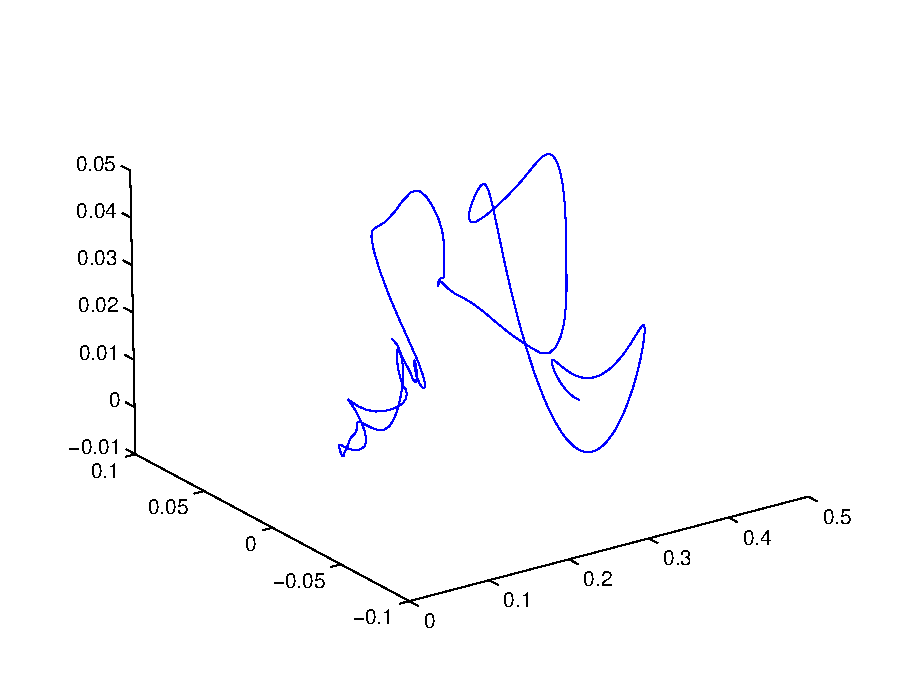
\includegraphics[width=2.5in]{UBef4}
 \caption{Trajectories along eigenfunctions from upper branch
  equilibrium
    (a) eigenfunction 1 file uUB1.ff need to remake
    (b) eigenfunction 2 file uUB2.ff need to remake
    (c) eigenfunction 3 file uUB3.ff need to remake
    (d) eigenfunction 4 file uUB4.ff
} \label{eltonFig:UBefs1/old}
\end{figure}

\begin{figure}[htbp]
  (e)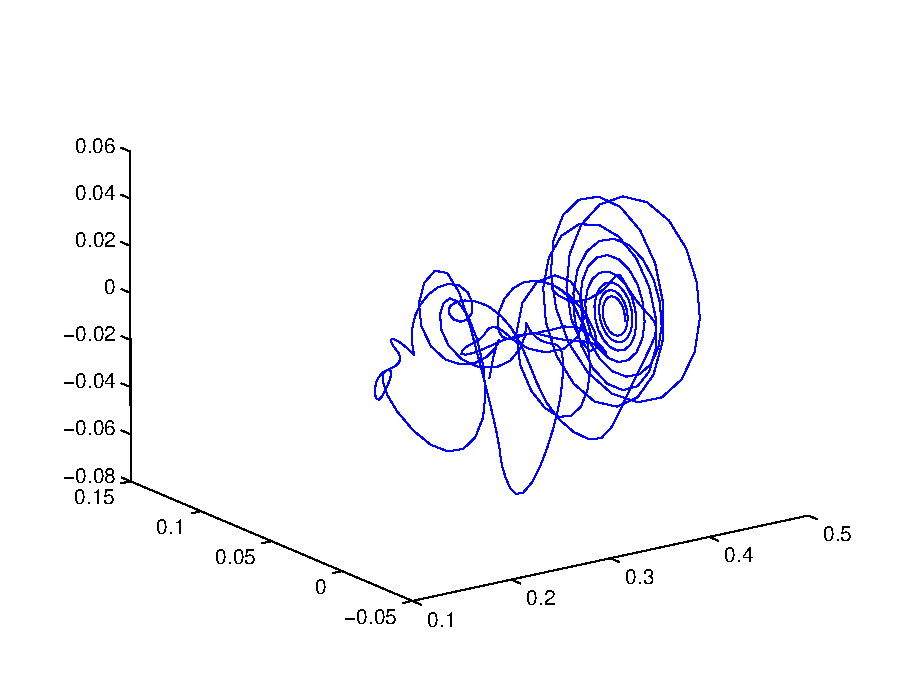
\includegraphics[width=2.5in]{UBef5}\\
  (f)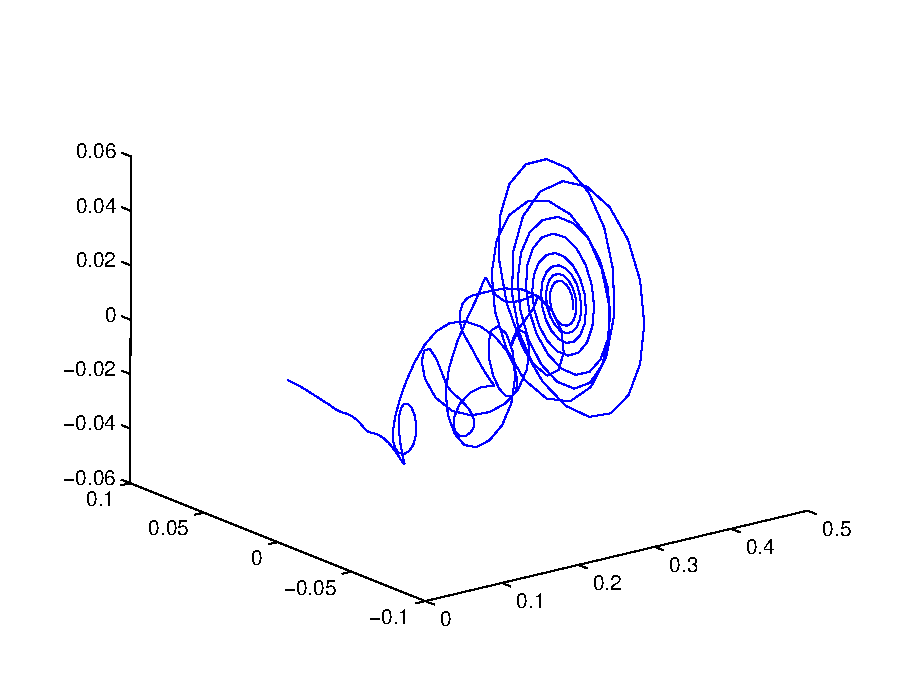
\includegraphics[width=2.5in]{UBef6}\\
  (g)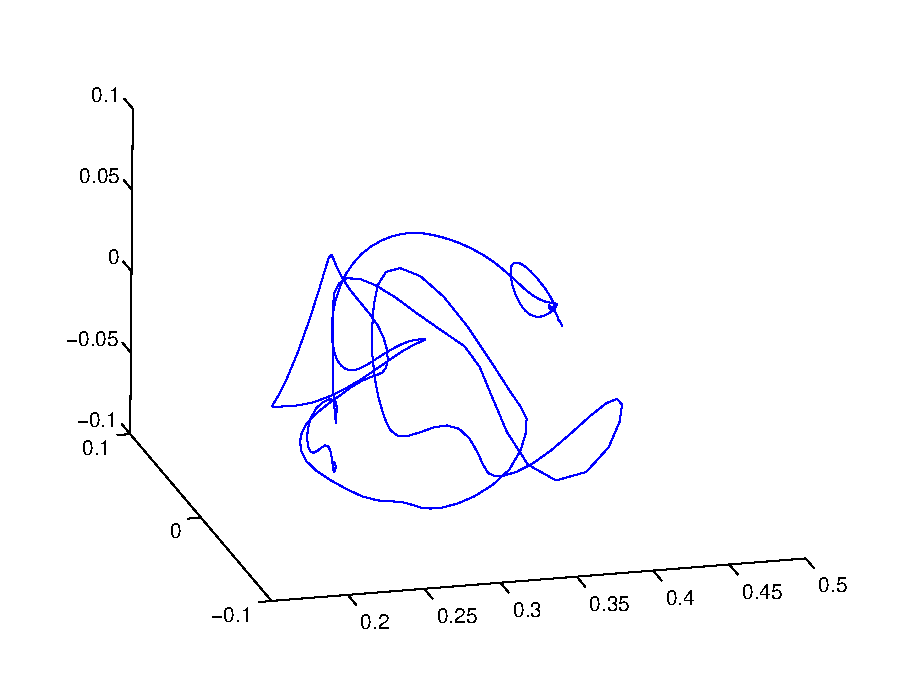
\includegraphics[width=2.5in]{UBef7}\\
  (h)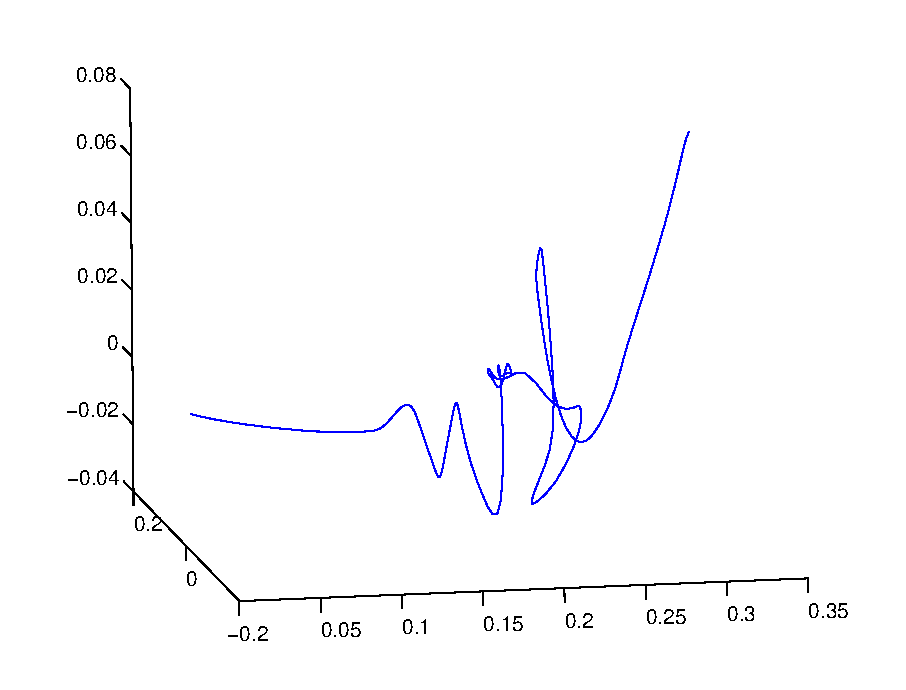
\includegraphics[width=2.5in]{uUB0}\\
  \caption{
  Trajectories along eigenfunctions from upper branch equilibrium
    (e) eigenfunction 5 file {\tt uUB5.ff}
    (f) eigenfunction 6 file {\tt uUB6.ff}
    (g) eigenfunction 7 file {\tt uUB7.ff}
    (h) eigenfunction 0 file {\tt uUB0.ff}
          }
  \label{eltonFig:UBefs2/old}
\end{figure}

% new eigenfunction figures
\begin{figure}[htbp]
  (a)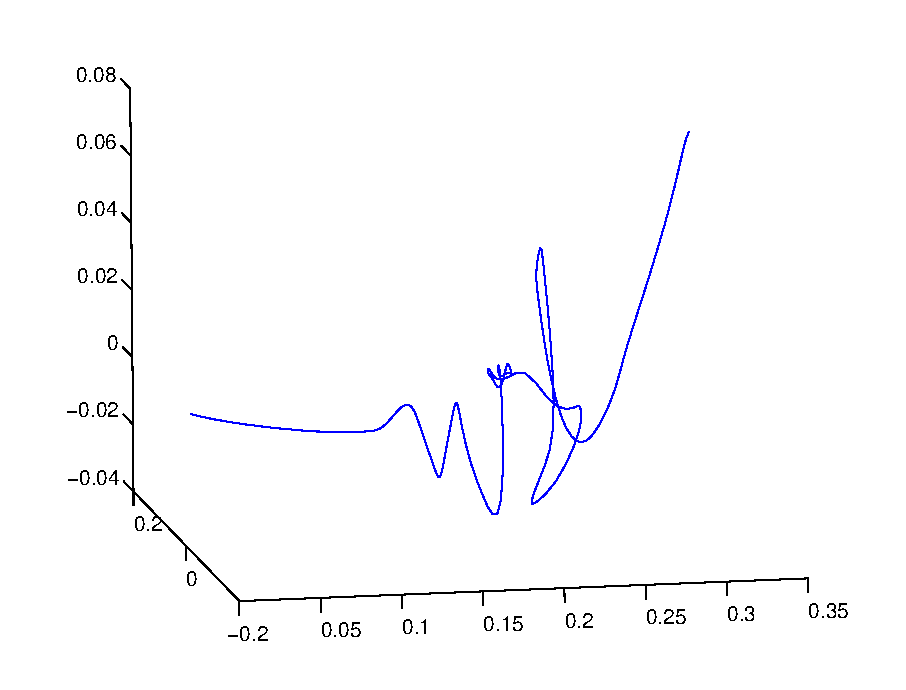
\includegraphics[width=2.5in]{uUB0}\\
  (b)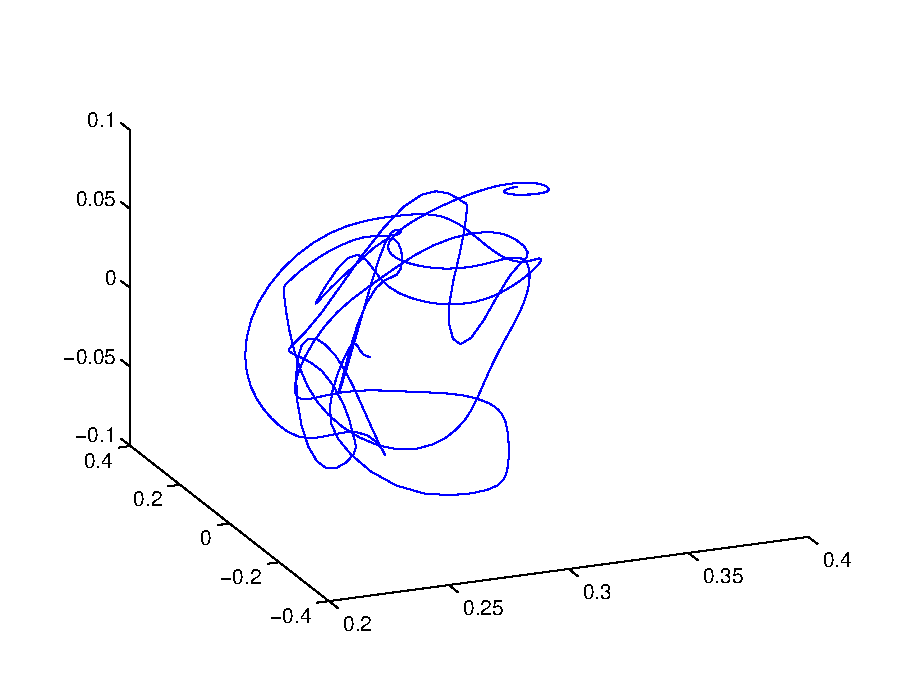
\includegraphics[width=2.5in]{uUB1}\\
  (c)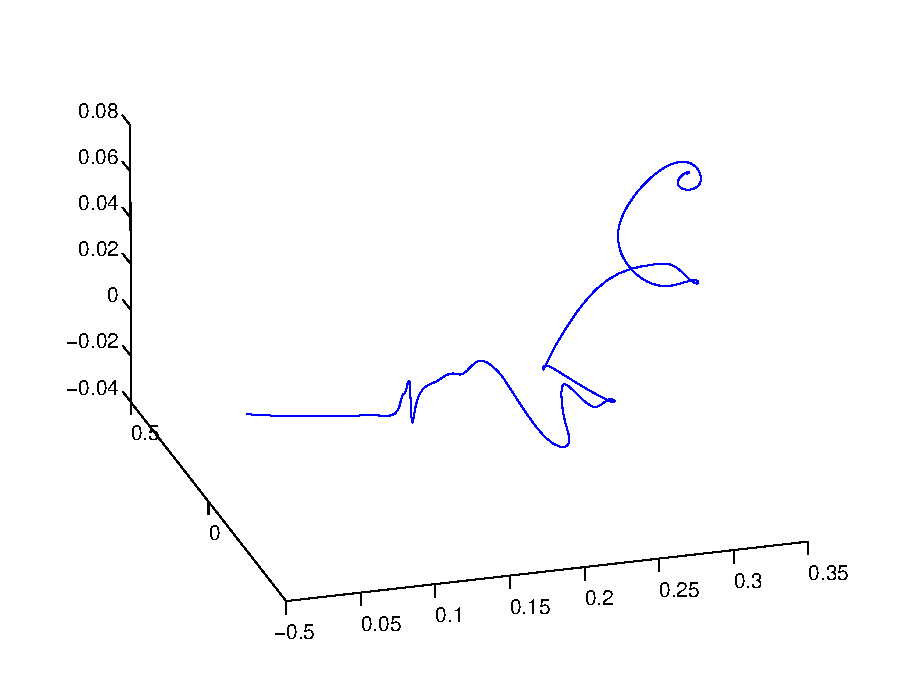
\includegraphics[width=2.5in]{uUB3}\\
  (d)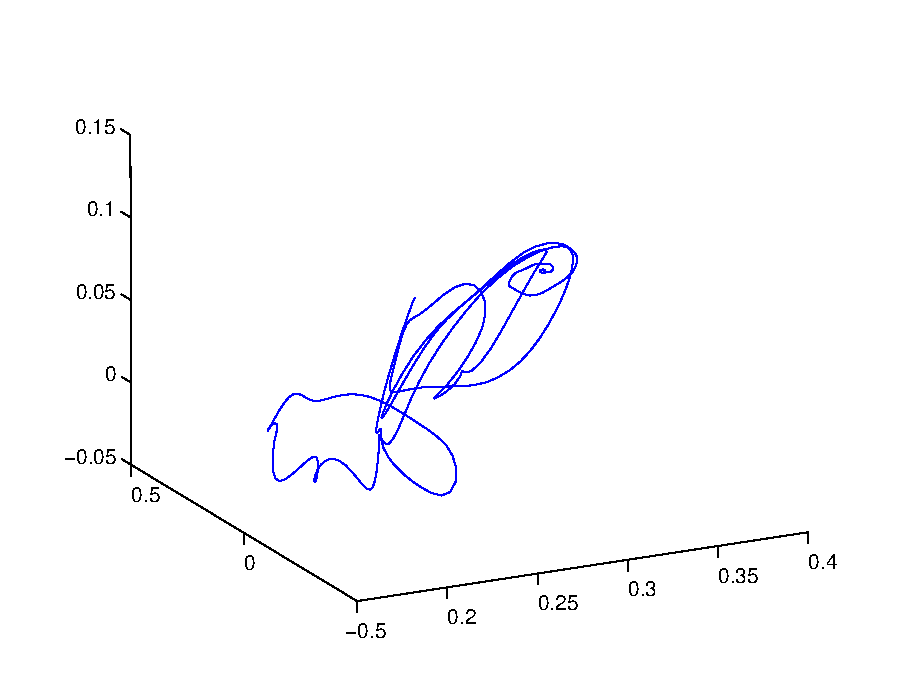
\includegraphics[width=2.5in]{uUB5}\\
 \caption{Trajectories along eigenfunctions from upper branch
  equilibrium
    (a) eigenfunction 0 file {\tt uUB0.asc}
    (b) eigenfunction 1 file {\tt uUB1.asc}
    (c) eigenfunction 3 file {\tt uUB3.asc}
    (d) eigenfunction 5 file {\tt uUB5.asc}
} \label{eltonFig:UBefs1/new}
\end{figure}

\begin{figure}[htbp]
  (e)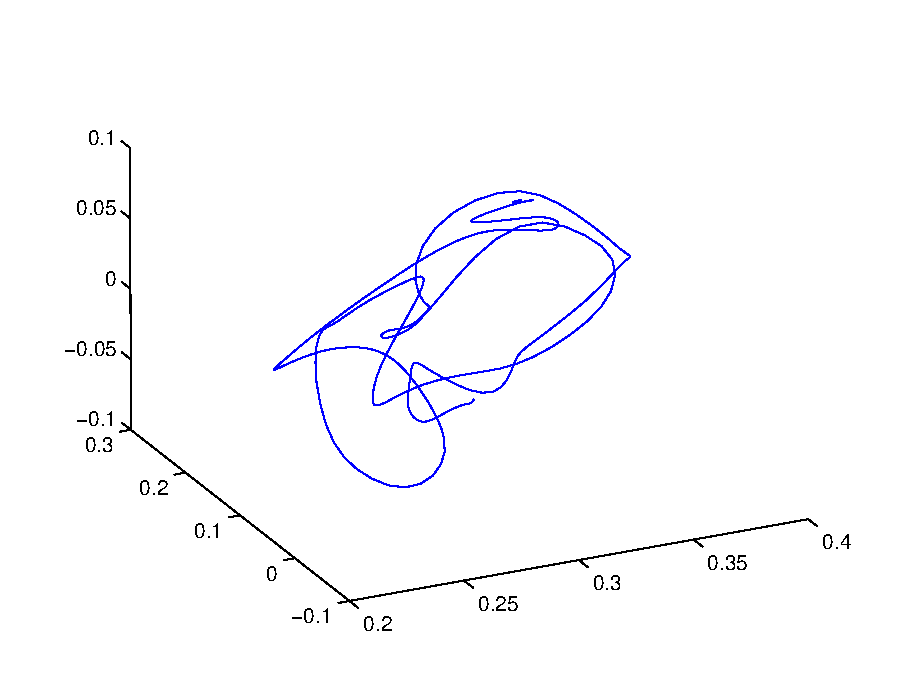
\includegraphics[width=2.5in]{uUB7}\\
  (f)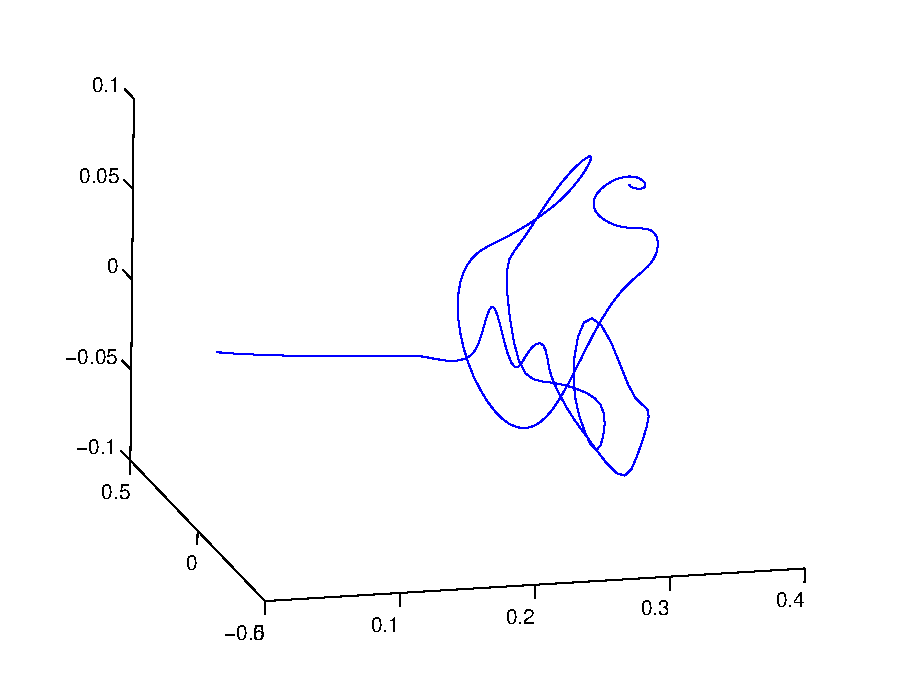
\includegraphics[width=2.5in]{uUB2}\\
  (g)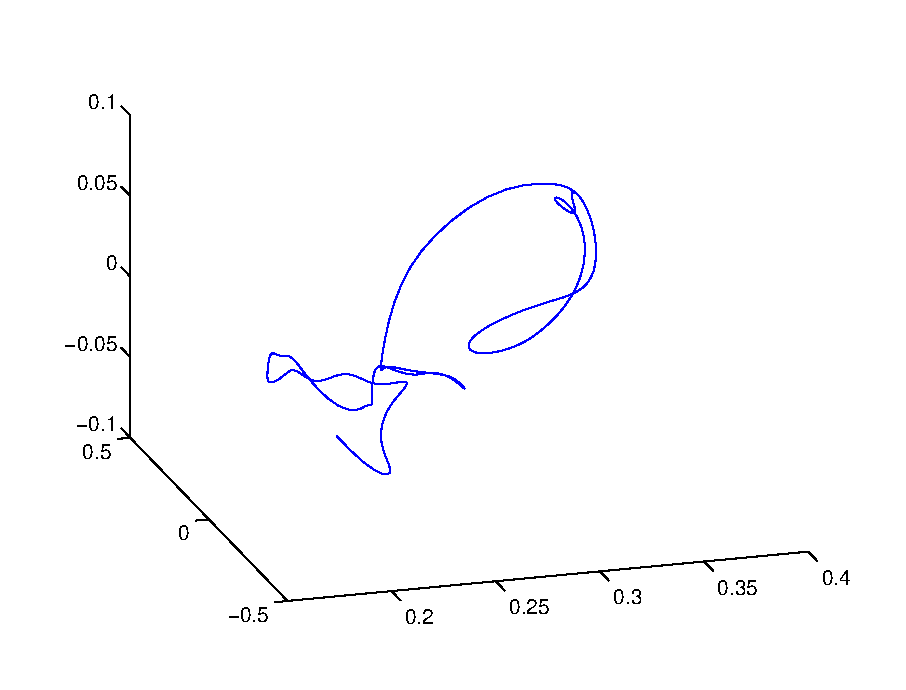
\includegraphics[width=2.5in]{uUB4}\\
  (h)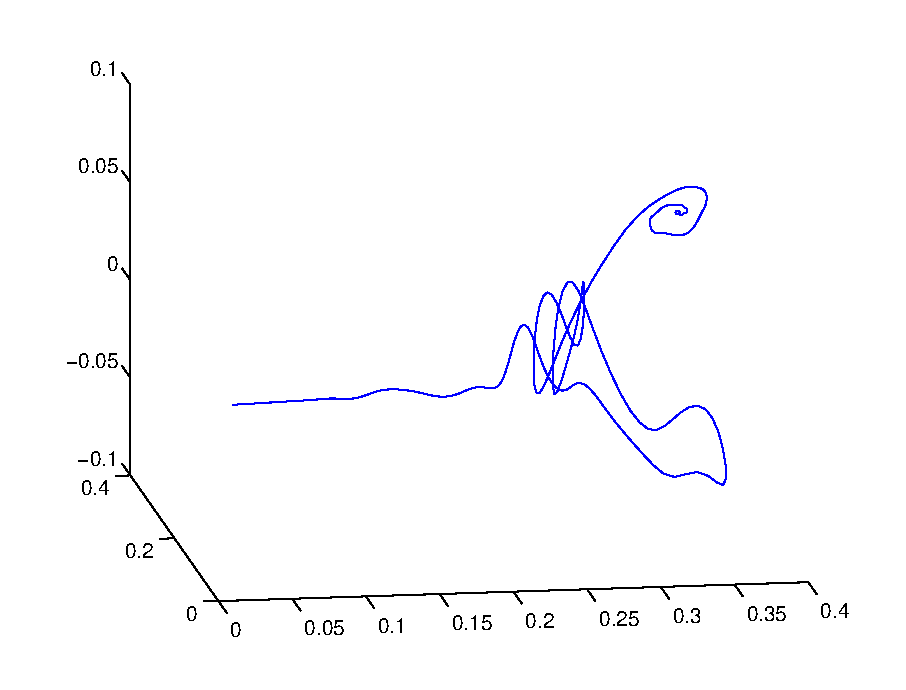
\includegraphics[width=2.5in]{uUB6}\\
  \caption{
  Trajectories along eigenfunctions from upper branch equilibrium
    (e) eigenfunction 7 file {\tt uUB7.asc}
    (f) eigenfunction 2 file {\tt uUB2.asc}
    (g) eigenfunction 4 file {\tt uUB4.asc}
    (h) eigenfunction 6 file {\tt uUB6.asc}
          }
  \label{eltonFig:UBefs2/new}
\end{figure}

\newpage
\newpage
\newpage
\newpage


\section{Discussion}
\label{sec:sum}

The preceding results summarize my efforts at discovering and
attaining information about the dynamics of plane Couette
turbulence. From the outset my approach has been to try something,
see what happens, and possibly adjust. The nature of the problem
forces this somewhat "hit or miss" technique. The most important
results produced in this way are the random initial condition
trajectories from \reffig{eltonFig:random2} and the trajectories
from equilibrium in figures
\reffigs{eltonFig:UBefs1/new}{eltonFig:UBefs2/new}. The 'knotted'
region in \reffig{eltonFig:random2} would probably be the most
interesting property to look at in future investigations. I would
like to have been able to draw more comparisons and conclusions
between my data and previously computed data from other sources, and
to give more results, but ultimately time and complexity of the
problem did not allow this. The methods set up would however provide
a nice starting point for a future investigation project by myself
or another. The method relies heavily on the use of all of the {\tt
channelflow} programs aforementioned as well as PCF data which has
already been compiled and analyzed. Numerical computation power is
therefore very important in investigating this problem.




\newpage
\section{Appendix: Some notes on fluids} \label{sec:fluids}

I have compiled some reference notes on the material which I have
been reading out of Lautrup~\cite{Lautrup} that can be referred back
to as a guide or quick reminder.

% This is also an exercise in equation writing with LATEX.

\subsection{Conservation of Mass}
\label{sec:ConsMass}
 The rate at which mass is gained in a volume V is equal to the rate
 of loss through its surface S.
 \beq
  \frac{d}{dt}\int{\rho dV} + \oint{\rho (\vec{v} \cdot \hat{n}) dS} =
  0
  \eeq
Using Gauss' Theorem, this can be reformulated as the continuity
equation, \beq
 \frac{\partial \rho}{\partial t} + (\vec{v} \cdot \nabla)\rho =
 -\rho \, \nabla \cdot \vec{v}
 \eeq
 For an incompressible velocity field the divergence of $v$ is 0 and
 a slightly simplified continuity equation can be used.
Defining the `material time derivative' as $\frac{D}{Dt} =
\frac{\partial}{\partial t} + \vec{v} \cdot \nabla$, the comoving
acceleration is given as
 \beq
 \frac{D \vec{v}}{D t} = \frac{\partial
\vec{v}}{\partial t} + (\vec{v} \cdot \nabla)\vec{v}
 \eeq
 The nonlinear term $(\vec{v} \cdot \nabla)\vec{v}$ is known as the
`convective'
 or `inertia' term.  It is the acceleration that is due to the
 material transporting the particle.  In cartesian coordinates it
 can be written as,
 \beq
(\vec{v} \cdot \nabla)\vec{v} = (v_{x} \frac{\partial
v_{x}}{\partial x})\hat{i} + (v_{y} \frac{\partial v_{y}}{\partial
y})\hat{j} + (v_{z} \frac{\partial v_{z}}{\partial z})\hat{k}
  \eeq
  For a steady flow, $\frac{\partial \vec{v}}{\partial t} = 0$ and
  the inertia term is the only source of acceleration.  Finally,
  from Newton's second law, we have Cauchy's equation of motion for a force
  density f:
  \beq
  f = \rho \left(
    \frac{\partial \vec{v}}{\partial t} + (\vec{v} \cdot \nabla)\vec{v}
        \right)
  \eeq
  The Cauchy equation is the governing equation for the motion of
  all fluids.

  \subsection{Viscosity, Reynolds Number \Reynolds, and Navier-Stokes}
\label{sec:Rey}

A fluid which flows along the $x$ axis with velocity $v(y)$ which is
independent of the coordinate $x$ is said to be laminar.  The shear
stress between layers due to friction is a measure of the viscosity
of the fluid.  The force density in Cauchy's equation is made up of
a pressure gradient and of the stress tensor, which incorporates a
viscosity term $\nu \nabla^{2} v$. $\nu$ is known as the kinematic
viscosity of the fluid.  Combining all of these terms and assuming
the density of the fluid to be constant we arrive at the
incompressible Navier-Stokes equations:
 \bea
 \frac{\partial \vec{v}}{\partial t} + (\vec{v} \cdot \nabla)\vec{v}
    &=&
 -\frac{1}{\rho}\nabla p + \nu \nabla^{2}v
    \label{NSe}\\
\nabla \cdot \vec{v}  &=& 0
    \label{incompr}
\,.
\eea
 The relation between the inertia of a fluid and its viscosity
 gives rise to the Reynolds Number
 \beq
 \Reynolds = \frac{\rho(\vec{v} \cdot \nabla)\vec{v}}{\eta \nabla^{2} v}
 \label{PCFRe}
 \eeq
 This ratio implies that large \Reynolds\ fluids flow freely while
small \Reynolds\ fluids are highly viscous.  For a flow between 2
plates separated by a distance $d$ (problem at
 hand) with average flow velocity $U$, the Reynolds number can be
 given as
\beq
 \Reynolds = \frac{U d}{\nu}.
\eeq









%%%%%%%%%%%%%%%%%%%%%%%%%%%%%%%%%%%%%%%%%%%%%%%%%%%%%%%%%%%%%



%%%%%%%%%%%%%%%%%%%%%%%%%%%%%%%%%%%%%%%%%%%%%%%%%%%%%%%%%%%%%

\bibliography{bibtex/elton}

\end{document}
